\documentclass[twoside]{../zirkelblatt1415}
\usepackage{float}
\usepackage{dashrule}
\usepackage{booktabs}
\floatstyle{ruled}
\restylefloat{figure}
\restylefloat{table}
\let\raggedsection\centering
\newcommand{\RR}{\mathbb{R}}

\theoremstyle{definition}
\newtheorem{defn}{Definition}[section]
\newtheorem{axiom}[defn]{Axiom}
\newtheorem{bsp}[defn]{Beispiel}

\theoremstyle{plain}

\newtheorem{prop}[defn]{Proposition}
\newtheorem{motto}[defn]{Motto}
\newtheorem{wunder}[defn]{Wunder}
\newtheorem{ueberlegung}[defn]{Überlegung}
\newtheorem{lemma}[defn]{Lemma}
\newtheorem{kor}[defn]{Korollar}
\newtheorem{hilfsaussage}[defn]{Hilfsaussage}
\newtheorem{satz}[defn]{Satz}
\newtheorem{thm}[defn]{Theorem}

\theoremstyle{remark}
\newtheorem{bem}[defn]{Bemerkung}
\newtheorem{aufg}[defn]{Aufgabe}

\definecolor{darkred}{rgb}{0.7,0,0}
\definecolor{shadecolor}{rgb}{.95,.95,.95}

\newenvironment{listing}{
  \renewcommand*\theenumi{\arabic{enumi}}
  \renewcommand{\labelenumi}{\theenumi.}
  \begin{enumerate}\itemsep0em}{\end{enumerate}}

\newcommand{\BB}{\mathrm{BB}}

\begin{document}

\maketitleCustom{Klassen 10/11/12}{\textbf{\textsf{%
  Gödels Unvollständigkeitssatz \\
  \normalsize Zirkelzettel vom 7. November 2014}}}

{\renewcommand{\addvspace}[1]{\vskip0.6em}
\tableofcontents%
}

\section{Einleitung}


\section{Berrys Paradoxon}


\section{Das Halteproblem}

Manche Computerprogramme stoppen nach endlich vielen Rechenschritten
("`halten"'), andere nicht. Etwa hält das Programm "`Lese vom Benutzer eine
Zahl ein, verdopple diese Zahl und gebe das Ergebis aus"', während das Programm
"`Gebe alle natürlichen Zahlen aus"' nicht hält. Im Allgemeinen ist es sehr
schwer, einem Programm anzusehen, ob es hält oder nicht.

\begin{bsp}\label{bsp:unklares-programm}Die \emph{Goldbachsche Vermutung}
besagt, dass jede gerade Zahl
größer als~2 die Summe zweier Primzahlen ist. Für jede
konkrete gerade Zahl~$n$ größer als~2 kann man das leicht überprüfen, indem man
einfach alle Paare von Primzahlen, die kleiner als~$n$ sind, durchgeht; etwa
sieht man durch Ausprobieren, dass~$14 = 3 + 11$ als Summe zweier Primzahlen
geschrieben werden kann. Noch ist die Vermutung im allgemeinen Fall aber ein
offenes Forschungsproblem. Daher ist nicht klar, ob folgendes Programm hält
oder nicht:
\begin{listing}
\item[1.] Beginne mit~$n := 4$.
\item[2.] Prüfe, ob~$n$ die Summe zweier Primzahlen ist.
\item[3.] Falls ja: Erhöhe~$n$ um Zwei und gehe zurück zu Schritt~2.
\item[4.] Falls nein: Halte.
\end{listing}
Dieses Programm hält genau dann, wenn es ein Gegenbeispiel zur Goldbachschen
Vermutung gibt.
\end{bsp}

\begin{bsp}Eine \emph{Fermatsche Primzahl} ist eine Primzahl der
Form~$2^{(2^n)} + 1$. Die Primzahlen~$3$, $5$, $17$, $257$ und~$65537$ sind von
diesem Typ (für~$n = 0,1,2,3,4$), aber es ist ein offenes Forschungproblem, ob
es weitere Fermatsche Primzahlen gibt. Daher ist von folgendem Programm nicht
klar, ob es hält:
\begin{listing}
\item[1.] Beginne mit~$n := 5$.
\item[2.] Prüfe, ob~$2^{(2^n)}$ eine Primzahl ist.
\item[3.] Falls ja: Halte.
\item[4.] Falls nein: Erhöhe~$n$ um Eins und gehe zurück zu Schritt~2.
\end{listing}
\end{bsp}

Beim \emph{Halteproblem} geht es darum, von einem gegebenen Programm
festzustellen, ob es hält oder nicht. Der britische Logiker, Mathematiker,
Kryptoanalytiker und Informatiker Alan Turing\footnote{Turing leistete während des
Zweiten Weltkriegs entscheidende Beiträge zur Kryptoanalyse der
deutschen Verschlüsselungsmaschine Enigma und ermöglichte so die
Entschlüsselung deutscher Funksprüche. Wegen seiner Homosexualität wurde er
im März~1952 zur chemischen Kastration verurteilt. Er erkrankte an
Depression und beging Suizid.} (*~1912, †~1954) bewies 1937, dass das Halteproblem
\emph{nicht entscheidbar} ist. Genau formuliert bedeutet das:

\begin{thm}Es gibt kein Programm, das bei Eingabe eines Programms~$P$ mit einer
korrekten Ausgabe von~"`$P$ hält"' oder~"`$P$ hält nicht"' hält.\end{thm}

Ein hypothetisches solches Programm wird auch \emph{Halteorakel} genannt.
Bemerkenswert an dem Theorem ist, dass es eine absolute Aussage trifft --
Turing behauptet nicht nur, dass \emph{wir} kein solches Halteorakel kennen.
Diese schwächere Behauptung ist auch gar nicht erstaunlich, erfordert doch im
Allgemeinen die Lösung des Halteproblems beliebige offene mathematische
Probleme zu lösen (Beispiel~\ref{bsp:unklares-programm}).
Vielmehr behauptet Turing, dass ein Halteorakel rein prinzipiell nicht
existieren kann. Auch Außerirdische mit überlegener Technologie oder
transzendente Wesen können kein Halteorakel programmieren.

\begin{bem}Programme können durchaus andere Programme simulieren. Das hilft
aber bei der (zum Scheitern verurteilten) Konstruktion eines Halteorakels
nicht: Wir können zwar ein gegebenes Programm~$P$ simulieren und, zum Beispiel,
10.000 Rechenschritte abwarten. Wenn~$P$ bis dahin aber nicht gehalten hat,
wissen wir immer noch nicht, ob~$P$ später halten wird oder nicht.
\end{bem}

\begin{bem}Einzelne Instanzen des Halteproblems können durchaus algorithmisch
lösbar sein,\footnote{Tatsächlich gibt es sogar für \emph{jedes} Programm~$P$
ein auf~$P$ maßgeschneidertes Orakelprogramm, welches korrekt die Meldung~"`$P$
hält"' oder~"`$P$ hält nicht"' ausgibt. Denn es ist ja klar, dass~$P$ entweder
hält oder nicht hält.  Im ersten Fall ist das triviale Programm, das sich
direkt nach seinem Aufruf mit der Meldung~"`$P$ hält"' sofort wieder beendet,
das gesuchte Halteorakel. Im zweiten Fall ist es das ebenso triviale Programm,
das die Meldung~"`$P$ hält nicht"' ausgibt. Die Situation wirkt vielleicht
etwas wundersam: Eines dieser beiden (trivialen!) Programme ist das gesuchte
Halteorakel, wir können nur im Allgemeinen nicht sagen, welches es ist.}
Turings Resultat sagt nur aus, dass es kein \emph{einzelnes}
Programm gibt, welche \emph{alle} Instanzen des Problems lösen kann -- welches
also bei Eingabe eines \emph{beliebigen} Programms in endlicher Zeit mit der
Meldung~"`hält"' oder~"`hält nicht"' terminiert.\end{bem}

\begin{table}[t]
  \begin{enumerate}
    \item[1.] \texttt{a}
    \item[2.] \texttt{b}
    \item[] $\vdots$
    \item[26.] \texttt{z}
    \item[27.] \texttt{aa}
    \item[28.] \texttt{ab}
    \item[] $\vdots$
    \item[41320.] \texttt{bice}
    \item[] $\vdots$
  \end{enumerate}
  \centering
  \caption{\label{tafel:liste-aller-programme}Ein Beispiel, wie die Liste aller
  Programme aussehen könnte, wenn die verwendete Programmiersprache nur die
  Zeichen~\texttt{a} bis~\texttt{z} verwendet.}
\end{table}

\begin{proof}[Beweis des Theorems]Als Vorbemerkung halten wir fest, dass wir
die Gesamtheit aller Programme in einer unendlichen Liste organisieren können
(Tafel~\ref{tafel:liste-aller-programme}) und darüber hinaus ein Programm~$F$
schreiben können, das bei Eingabe einer natürlichen Zahl~$n$ das~$n$-te
Programm dieser Liste ausgibt.

Angenommen, es gibt ein Halteorakel~$H$.\footnote{Eigentlich müssen wir den
Rest des Beweises in den Konjunktiv setzen, da wir ab dieser Stelle eine Annahme
treffen (mit dem Ziel, einen Widerspruch zu erkennen, um die Falschheit
der Annahme nachzuweisen). Das ist aber umständlich.}
Dann können wir ein Programm~$R$
programmieren, das wie folgt abläuft:
\begin{listing}
\item Lese eine Zahl~$n$ als Eingabe ein.
\item Lasse das Halteorakel ablaufen, um herauszufinden, ob das
Programm~$F(n)$ (also das~$n$-te Programm auf der Liste) bei Eingabe von~$n$
hält oder nicht.
\item Falls es hält: Gehe in eine Endlosschleife.
\item Falls es nicht hält: Halte.
\end{listing}
Das Programm~$R$ zeigt bei Eingabe von~$n$ also genau das entgegengesetzte
Halteverhalten von~$F(n)$.

Wie jedes Programm ist auch~$R$ in der Liste aller
Programme verzeichnet, etwa an~$m$-ter Stelle: Es gilt also~$F(m) = R$.
Wir können uns nun fragen, ob~$R$ bei Eingabe von~$m$ hält oder nicht. Verfolgen
wir den Programmfluss, sehen wir aber, dass beide Fälle zu einem Widerspruch
führen.
\end{proof}

\begin{aufgabeShaded}{Verstanden?}
\begin{enumerate}
\item Vollziehe den Beweis des Theorems nach. Könntest du jemand anderem
erklären, welche Widersprüche die Existenz eines Halteorakels nach sich ziehen
würde?
\item Wieso war es für den Beweis wichtig, dass es das Programm~$F$ gibt? Wieso
also war es wichtig, dass wir bei Eingabe einer Zahl~$n$ das~$n$-te Programm
auf der Liste aller Programme berechnen können?
\end{enumerate}
\vspace{-1em}
\end{aufgabeShaded}

Was ist eigentlich ein \emph{Programm}? Auf diese Frage sollten wir eine
präzise Antwort haben, wenn wir rigoros Mathematik betreiben möchten. Zur
Vorstellung ist es -- insbesondere, wenn man Programmiererfahrung hat --
hilfreich, sich Programme einer realen Programmiersprache (Haskell, Perl,
Python, \ldots) vorzustellen, welche aber auf \emph{idealisierten Computern}
ablaufen: Computer, die niemals kaputt gehen und über beliebig viel
Arbeitsspeicher verfügen.

Um diese Vorstellung aber zu präzisieren, hat Turing das nach ihm benannte
Konzept der \emph{Turingmaschine} entworfen. Turingmaschinen sind abstrakte
Rechenmaschinen, die sich, weil sie von den vielen Details realer Computer
abstrahieren, für mathematische Untersuchungen besonders gut eignen. Mit
\emph{Programm} meinen wir also eigentlich \emph{Turingmaschine}.

Eine Turingmaschine arbeitet auf einem in beide Richtungen unendlich langem
Band, dessen Zellen die Werte~0 und~1 fassen können
(Abbildung~\ref{abb:turing-maschine}).  In jedem Rechenschritt kann die
Turingmaschine den gespeicherten Wert auf dem Band an der aktuellen Position
lesen, einen neuen Wert schreiben und das Band um eine Zelle nach links oder
rechts verschieben. Dabei befolgt sie ein für sie eindeutiges, endliches
Regelwerk.

\begin{aufgabeShaded}{Das Halteproblem für halbreale Computerprogramme}
In dieser Aufgabe soll es um Programme gehen, die auf Computern laufen, welche
zwar nie kaputt gehen und auch nicht aufgrund äußerer Einflüsse in ihrem
Verhalten gestört werden (etwa durch kosmische Strahlung), aber trotzdem nur
über endlichen Speicher verfügen. Außerdem sollen sie von der Außenwelt in dem
Sinn isoliert seien, dass sie etwa keine Verbindung zum Internet besitzen.
Kurz und präzise, aber vielleicht weniger anschaulich: Es soll um
Turingmaschinen mit endlichem Band gehen.

Erkläre, wieso das Halteproblem für solche Programme (zumindest in der
Theorie) trivial lösbar ist.

\emph{Tipp:} In wie vielen verschiedenen Zuständen kann sich ein derartiger
Computer befinden?
\end{aufgabeShaded}

\begin{aufgabeShaded}{Der Satz von Rice}
Der \emph{Satz von Rice} ist eine Verschärfung von Turings
Unmöglichkeitstheorem. Er besagt: Für keine nichttriviale extensionale
Programmeigenschaft~$E$ gibt es ein Orakel, das bei Eingabe
eines Programms~$P$ mit einer korrekten Ausgabe von~"`$P$ hat Eigenschaft~$E$"'
oder~"`$P$ hat Eigenschaft~$E$ nicht"' hält.

Dabei meint \emph{nichttrivial}, dass manche Programme die Eigenschaft~$E$
haben und andere nicht. Etwa ist die Eigenschaft~"`$P$ hält oder hält nicht"'
ein Beispiel für eine Eigenschaft, welche \emph{nicht} nichttrivial ist.

\emph{Extensionalität} verlangt, dass sich die Eigenschaft~$E$ nur auf das von
außen sichtbare Verhalten des Programms, nicht aber seine innere Struktur
(seinen Quellcode) bezieht. Etwa sind die Eigenschaften~"`$P$ hält"',
"`$P$ gibt als Ergebnis die Zahl~37 aus"' und "`$P$ gibt eine gerade Zahl als
Ergebnis aus"' extensionale Eigenschaften. Keine extensionalen Eigenschaften
sind~"`$P$ besteht aus weniger als~20 Zeilen Code"' und~"`$P$ tätigt
mindestens~100 Rechenschritte"'.

\begin{enumerate}
\item Überlege, wieso es ganz einfach ist, ein Orakel zu programmieren, dass
die nicht-extensionale Eigenschaft~"`$P$ besteht aus weniger als~20 Zeilen
Code"' prüft.
\item Beweise den Satz von Rice. Du kannst dich dabei am Beweis der
Unentscheidbarkeit des Halteproblems orientieren.
\end{enumerate}
\vspace{-1em}
\end{aufgabeShaded}

\begin{aufgabeShaded}{Die Church--Turing-These}
Informiere dich auf Wikipedia, was es mit der Church--Turing-These auf sich
hat; manche Leute halten sie für eine der größten ungeklärten Fragen der Physik
und Informatik. Hast du eine Meinung dazu?
\end{aufgabeShaded}

\begin{figure}[h]
  \centering
  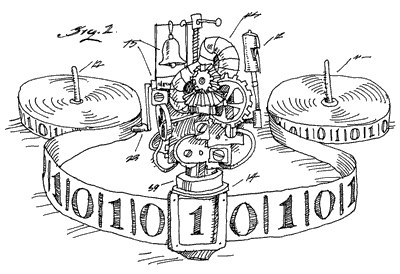
\includegraphics[scale=0.7]{turing-machine}
  \caption{\label{abb:turing-maschine}Eine künstlerische Darstellung einer
  Turing-Maschine. Quelle:
  \url{http://www.worldofcomputing.net/wp-content/uploads/2013/01/turingMachine.gif}}
\end{figure}


\section{Die unberechenbare Fleißiger-Biber-Funktion}

\emph{Dieser Abschnitt wird noch ausgebaut. Wer möchte, kann sich aber schon
vorab mit der Aufgabe beschäftigen.}

Die \emph{Fleißiger-Biber-Funktion} ist eine Funktion~$\BB : \NN \to \NN$, die
eng mit dem Halteproblem verknüpft ist. Per Definition ist~$\BB(n)$ die größte
Anzahl Rechenschritte, die irgendein haltendes Programm mit
Quelltextlänge~$\leq n$ macht.

Anders formuliert: Unter den Programmen mit Länge~$\leq n$ gibt es welche, die
halten, und welche, die nicht halten. Unter denen, die halten, gibt es ein
Programm, dass unter all diesen Programmen am meisten Rechenschritte ausführt,
bevor es schlussendlich hält. Die Anzahl dieser Rechenschritte ist~$\BB(n)$.

Die exakten Werte der Fleißiger-Biber-Funktion hängen von der Wahl der
Programmiersprache ab, denn in verschiedenen Sprachen drückt man sich beim
Programmieren unterschiedlich aus. In der Literatur verwendet man daher die
abstrakten Turingmaschinen als Referenzpunkt.

Die Fleißiger-Biber-Funktion wächst rasant an, viel schneller als exponentiell;
nur sehr wenige Funktionswerte sind bekannt (Tabelle~\ref{tab:bb}). Tatsächlich
wächst sie (asymptotisch) \emph{schneller als jede durch Programme berechenbare
Funktion}. Wie auch bei Turings Unmöglichkeitsresultat liegt der Grund dafür
nicht in menschlichen technologischen Beschränkungen, sondern ist
prinzipieller Natur.

\begin{table}
  \begin{tabular}{@{}lll@{}}
    \toprule
    $n$ & Anzahl Programme der Länge~$\leq n$ & $\BB(n)$ \\\midrule
    1 & 64 & 1 (1962) \\
    2 & 20736 & 4 (1962) \\
    3 & 16777216 & 6 (1965) \\
    4 & $25{,}6 \cdot 10^9$ & 13 (1972) \\
    5 & $\approx 63{,}4 \cdot 10^{12}$ & $\geq 4098$ (1989) \\
    6 & $\approx 232 \cdot 10^{15}$ & $> 3{,}514 \cdot 10^{18267}$ (2010) \\
    \bottomrule
  \end{tabular}
  \centering
  \caption{\label{tab:bb}Die bekannten Werte der Fleißiger-Biber-Funktion. Mit
  \emph{Programm} ist hier \emph{Turingmaschine} und mit \emph{Länge}
  die Anzahl der Zustände gemeint. Quelle:
  \url{http://de.wikipedia.org/wiki/Fleißiger_Biber}}
\end{table}

\begin{thm}Die Fleißiger-Biber-Funktion ist nicht berechenbar, d.\,h. es gibt
kein Programm~$P$, das bei Eingabe einer natürlichen Zahl~$n$ die Zahl~$\BB(n)$
zurückgibt.\end{thm}

\begin{aufgabeShaded}{Unberechenbarkeit der Fleißiger-Biber-Funktion}
Beweise das Theorem, indem du folgende Argumentation ausformulierst:

Wenn es ein Programm gäbe, dass die Fleißiger-Biber-Funktion
berechnen könnte, dann könnte man daraus ein Halteorakel konstruieren (wie geht
das?). Dass es ein solches nicht gibt, wissen wir schon.
\end{aufgabeShaded}

\section{Chaitins Haltewahrscheinlichkeit}

\begin{quote}
Die Zahl~$\Omega$ verkörpert eine enorme Menge an Wissen auf sehr kleinem Raum.
Die ersten paar Tausend Ziffern, die problemlos auf einem kleinen Stück Papier
Platz finden könnten, enthalten die Antworten auf mehr mathematische Fragen,
als man im ganzen Universum aufschreiben könnte.

Im Laufe der Menschheitsgeschichte haben Mystiker und Philosophen nach einem
kompakten Schlüssel zu universeller Weisheit gestrebt, einer endlichen Formel
oder einem Text, der, wenn bekannt und verstanden, Antworten auf alle Fragen
liefern würde. Das Studium der Bibel, des Korans oder des I~Gings, um
Weissagungen zu treffen, illustriert diesen Glauben oder Hoffnung.

Solche Quellen universeller Weisheit sind herkömmlicher Weise vor beiläufigem
Zugriff geschützt: indem sie schwer zu finden, wenn gefunden schwierig zu
verstehen und gefährlich zu benutzen sind, dazu neigend, mehr und
tiefere Fragen zu beantworten als sich der Sucher wünschte. Das esoterische
Buch ist, wie Gott, einfach und dennoch unbeschreibbar. Es ist allwissend, und
verändert alle, die es kennen.

$\Omega$ ist in vielerlei Hinsicht eine kabbalistische Zahl. Dem menschlichen
Verstand ist sie bekannt, aber unkennbar. Um sie im Detail zu wissen, müsste
man ihre unberechenbare Ziffernfolge als Glaubensgrundsatz akzeptieren, so wie
die Worte eines heiligen Texts.
\end{quote}

\section{Formale Systeme und Modelle}

\section{Gödels Vollständigkeitssatz und sein Unvollständigkeitssatz}

\end{document}


=== Chaitins Haltewahrscheinlichkeit

* Zitat (C. H. Bennett)

  Omega comes from the Chaitin Omega Number, that "embodies an enormous amount
  of wisdom in a very small space ... inasmuch as its first few thousand
  digits, which could be written on a small piece of paper, contain the answers
  to more mathematical questions than could be written down in the entire
  universe.
  
  Throughout history mystics and philosophers have sought a compact
  key to universal wisdom, a finite formula or text which, when known and
  understood, would provide the answer to every question. The use of the Bible,
  the Koran and the I Ching for divination and the tradition of the secret
  books of Hermes Trismegistus, and the medieval Jewish Cabala exemplify this
  belief or hope.
  
  Such sources of universal wisdom are traditionally protected from casual use
  by being hard to find, hard to understand when found, and dangerous to use,
  tending to answer more questions and deeper ones than the searcher wishes to
  ask. The esoteric book is, like God, simple yet undescribable. It is
  omniscient, and transforms all who know it.

  Omega is in many senses a cabalistic number. It can be known of, but not
  known, through human reason. To know it in detail, one would have to accept
  its uncomputable digit sequence on faith, like words of a sacred text.

* Omega := sum_p 2^{-|p|}

* Kennt man die ersten N Bits von Omega, so kann man das Halteproblem für
  alle Programme der Länge <= N lösen:

  * Lasse alle Programme dieser Länge in verzahnter Art und Weise ablaufen.
  * Gelegentlich halten solche simulierten Programme an.
  * Warte so lange, bis sum_{p bis jetzt gehalten} 2^{-|p|} >= bekannte
    untere Schranke für Omega. (Das dauert nur endlich lange.)
  * Hat das gegebene Programm bis jetzt gehalten?
    Wenn ja: Es hält.
    Wenn nein: Es wird nie halten. Denn wenn doch, dann

        Omega >= sum_{bis jetzt} + 2^{-|p_0|} >= Omega + ... > Omega, Widerspruch.

* Diskussion des Zufallscharakters von Omega: Programme, die die ersten N
  Stellen von Omega ausgeben, können nicht kurz sein. (Anders als bei pi und
  Konsorten!)

  Motivieren durch:
  * Bilder von Fraktalen
  * Bild einer Ziffernfolge, die systematisch aufgebaut ist
  * Bild einer zufälligen Ziffernfolge (ha!)

* Diskussion der Flüchtigkeit von Omega: Kann Aussagen über Ziffern nicht beweisen.

* Unbedingt referenzieren:
  Grenzen der Mathematik: Eine Reise durch die Kerngebiete der mathematischen
  Logik, Dirk W. Hoffmann.


=== Formale Systeme und Modelle

* Ein formales System besteht aus einer Ansammlung von Axiomen und zulässigen
  logischen Schlussregeln.

* Ein Modell für ein formales System ist eine Struktur, in der die Axiome
  und Schlussregeln den Systems gelten.

* Schreibweisen:
  1. S |- phi
  2. M |= phi
  3. S |= phi

* Beispiel: Peano-Arithmetik mit den gewöhnlichen natürlichen Zahlen als
  intendiertes Modell

* Beispiel: wie nichtstandard Modelle der natürlichen Zahlen aussehen.


=== Gödels Sätze

* Vollständigkeitssatz: Wenn S |= phi, dann auch S |- phi.

* Unvollständigkeitssatz: Es gibt phi mit N |= phi, aber nicht PA |- phi.

* Beispiele für Gödel-Sätze:

  * "Dieser Satz hat keinen Beweis."
  * Goodstein-Folgen
  * Aussagen über Ziffern von Omega

* Currys Paradox!
